ss[11pt]{article}
\usepackage{graphicx}
\usepackage{amssymb}
\usepackage{epstopdf}
\usepackage{mystyle}
\usepackage{bm}
\usepackage{amsmath}
\DeclareGraphicsRule{.tif}{png}{.png}{`convert #1 `dirname #1`/`basename #1 .tif`.png}

\title{Trajectory guided gaussian basis method}
\author{Bing Gu}
%\date{}                                           % Activate to display a given date or no date

\begin{document}
\maketitle
\section{Gaussian Basis}
One possible way to solve time-dependent \se is to expand the initial wavepacket as a linear combination of basis functions. Gaussian basis with fixed width is becoming popular in recent years. 
\be g_{m}(x,t) = \sqrt[4] {\frac{a}{\pi}} \exp\left (-\frac{\alpha}{2}(x-q_{m}(t))^{2}+\im p_{m}(t)(x-q_{m}(t) \right) \ee 
\be |\psi_{0} \ket= \sum_{n=1,...,N}c_{n}(t=0)|g_{n}(q_{n},p_{n},t=0) \ket  \ee
\be \bra g_{m} | \psi_{0} \ket = \sum_{n}  c_{n}\bra g_{m} | g_{n} \ket, ~~~ m=1,...,N. \ee
where $N$ is the number of basis used to project the initial wavepacket. \\ 


Initial coefficients $c_{n}(0)$ can be obtained by solving the matrix equation 
\be \bf{M}\bm{c} =  \bm{b} \ee  
where 
\be {\bf M}_{mn} = \bra g_{m} | g_{n} \ket, ~~~{\bf b} = \{ \bra g_{1}  | \psi_{0} \ket, \dots , \bra g_{n} | \psi_{0} \ket \}. \ee 
%\subsection{}
Normalization of the wavepacket is conversed in the propagation.
\be N = \bra \psi | \psi \ket = \sum_{mn} \int dx ~\bm c_{m}^{*}{\bf M}_{mn}\bm c_{n}, \ee
\be \frac{dN}{dt} = 0 \ee 
It can be proved by using the Hermitian property of hamiltonian ${\bf H}$. 
%(\bm{c^{*}})^{T}\bm({\phi}^{*})^{T}\bm{\phi} \bm c = (\bm c^{*})^{T} \bf{M} \bm c \ee
Define 
\be \bm c = \{ c_{1}, c_{2},\dots, c_{N} \} \ee 
and 
\be \bm{ \phi} = \{ g_{1}(q_{1},p_{1}),\dots, g_{N}(q_{N},p_{N}) \}, \ee 
Wavefunction at time $t$ can be written as 
\be \psi(x,t) = \bm c^{T}(t)\bm \phi(t) \label{eq:expand} \ee  
if we substitute Eq. (\ref{eq:expand}) into time-dependent \se, propagation of the initial wavepacket can be transformed into the evolution of the coefficients $c_{n}(t)$ and the motion of $(p_{n}(t),q_{n}(t))$ of gaussian wave packets. 
The equations for evolution of $\bm c$ will be 
\be \im {\bf M} \dot{c} = ({\bf H} - \im \dot{\bf M})\bm c , \label{eq:dcdt} \ee 
where 
\be \dot{\bf M}_{mn} = \bra g_{m} | \dot{g_{n}} \ket \ee 
and ${\bf H}$ is the hamiltonian matrix,   
\be   {\bf H}_{mn} = \bra g_{m} | -\frac{\hbar^{2}}{2m}\grad^{2} + V(x) | g_{n} \ket . \ee
Potential energy is expanded into second-order Taylor series at  position of each trajectory
\be V(x) = V(q_{n}) + \grad V(q_{n} ) (x-q_{n}) + \frac{\grad^{2} V(q_{n})}{2}(x-q_{n})^{2} + O((x-q_{n})^{3}) \label{eq:taylor} \ee 
Substituting Eq. (\ref{eq:taylor}) to Eq. (\ref{eq:dcdt}) and ignore the third-order term, we will obtain 
\be {\bf H}_{mn} = \bra g_{m} | d_{0}+d_{1}(x-q_n)+d_{2}(x-q_n)^2 | g_{n} \ket . \ee
\be d_{0} = V(x_{n}) - \frac{p^{2}_{n}-\alpha}{2m},~~d_{1} = -\grad U(x_{n}), ~~ d_{2} = \frac{1}{2} \left (\grad^{2}V(x_{n}) - \frac{\alpha^{2}}{m} \right) \ee 

\section{System}
Quantum effects can be incorporated into the dynamics of parameter trajectories of gaussian basis.
At first beginning, linear quantum force(LQF) is being used to the evolution of trajectories, and 
Morse Oscilator for $H_2$ is being tested. 
The initial wavefunction is set as 
\be \psi(x,0) = \sqrt[4]{\frac{2\alpha_0}{\pi}}\exp(-\alpha_0(x-x_0)^2+\im p_0(x-x_0)) \ee 
We set $x_0 = 1.4,~ \alpha_0=9.16$. Atomic units are used if not specified throughtout the paper.

Because of the inefficiency of LQF of quantum trajectories, some trajectories will diverge. We introduce a parameter $cutoff$ to solve this problem. 
Trajectories which run out of $cutoff$ ($x(i) > cutoff$) are abondoned. 
  
%\begin{figure}[h]
%  \centering
%   \includegraphics[width=0.8\textwidth]{/home/bing/fg/spo_1d/wf}
%   \caption{Exact wavepacket propagation by Split-Operator method.}
%   \label{fig:spo}
%\end{figure}

%\begin{figure}[h]
%  \centering
%   \includegraphics[width=0.8\textwidth]{/home/bing/fg/lqf/wf}
%   \caption{Wave function at different times by quantum trajectories with LQF.}
%   \label{fig:lqf}
%\end{figure}

%\begin{figure}[h]
%  \centering
%   \includegraphics[width=0.8\textwidth]{/home/bing/fg/lqf_cut3/wf}
%   \caption{Wave function at different times with $cutoff = 2.5$.}
%   \label{fig:lqf_cut}
%\end{figure}
%
%\vspace{5inch}
%
%\begin{figure}[h]
%  \centering
%   \includegraphics[width=0.8\textwidth]{/home/bing/fg/lqf/ener}
%   \caption{Energy without $cutoff$.}
%   \label{fig:lqf_cut}
%\end{figure}
%
% \begin{figure}[h]
%  \centering
%   \includegraphics[width=0.8\textwidth]{/home/bing/fg/lqf_cut4/ener}
%   \caption{Energy with $cutoff=2.5$.}
%   \label{fig:lqf_cut}
%\end{figure}

\section{Approximate the wavefunction at each time step with one guassian}
Approximate $\psi(x,t)$ with one guassian $g(\alpha(t),x_0(t))$ at each time step. 
Fitting with a guassian is transformed into fitting $ln\psi(x,t)$ polynomials $f(x) = ax^2+bx+c$

Instead of using the classical force at the center of gaussian wavepacket, 


\newpage
\section{Ehrenfest trajectories}
Ehrenfest trajectories was firstly brought out to prevent trajectories from crossing as it averages the force acted on every 
trajectory. Each Ehrenfest trajectory is experiencing the same force. Quantum tunnelling effects is covered in a different way, 
but Ehrenfest approximation won't delocalize the wavefunction.
The equations of motion (EOM) for Ehrenfest trajectories are as follows:
\be \dot{q} = \frac{p}{m} \ee 
\be \dot{p} = \bra -\frac{\partial V}{\partial x} \ket \ee 


\section{Problems}
To describe a scattering system, the transmitted wavefunction will be spread out in space, wich is difficult to describe with few sharp gaussians.  

\section{Probability expansion - Another way to update coefficients}
In de Broglie-Bohm formulation of quantum mechanics, there are two coupled equations, one is the so-called quantum Hamilton-Jacobi equation(QHJE), the other is continuity equation. 
QHJE defines ``exact'' quantum trajectories, moving under external ``real'' force and  ``virtual'' quantum force, except for coherent state under harmonic well, where quantum potential is a constant, i.e. wavefunction keeps its shape through propagation. 

Computation of exact quantum potential needs the knowledge of the amplitude of wavefunction, which is extremely hard to compute numerically. Certain approximations has to be made about the ``hard'' term. 

On the other hand, continuity equation defines the weight of quantum trajectories, which is a constant i.e. no time dependence,  in Lagrangian frame of reference.  

Continuity equation in principle is a way to propagate density. So we can expand $\rho(x,t)$ in terms of basis functions $\phi(x;x_i)$, which is decided by the position of evolving trajectories $x_i$,

\be \rho(x,t) = \sum_i c_i \phi_(x;x_i) \ee 
If we substitute this expansion into continuity equation, we will obtain 
\be \sum_i \dot{c_i} \phi_{ji} +\sum_i c_i \bra \phi_j | \grad v | \phi_i \ket = 0 \ee  
where 
\be \phi_{ji} = \bra \phi_j | \phi_i \ket \ee 
We can propagate this equation simultaneously while evolving quantum trajectories with linear quantum force (LQF).  
If written in matrix form, we will get 
\be {\bf M}{\bm \dot{c}} = - {\bf G}\bm c \ee
where 
\be M_{ji} =   \bra \phi_j | \phi_i \ket, ~~G_{ji} = \bra \phi_j | \frac{\grad p}{m} | \phi_i \ket \ee
Matrix $G$ elements cannot be obtained directly, it seems necessary to do a polynomial (or other basis) fitting to get derivative of momentum, we can also add an equation of motion for the first-order derivative to the propagation, but then we need second-order derivative of potential, which is also hard to get. 

\section{Complex quantum trajectory approach} 
Complex Hamilton-Jacobi equation 
\be \psi(x,t) = \exp \left(\frac{\im}{\hbar}S(x,t)\right) \ee 

\be S_t + \frac{S_x}{2m}+V = \frac{\im \hbar}{2m}S_{xx} \ee 

\section{ideas}

quantum potential for excites states will not have ``bad'' singular points, i.e. quantum potential does not go to infinity at those nodes.
So if we have a constraint form to represent wavefunction, we may be able to get excited energy.

Questions: 
1) does quantum trajectories stop at excited states?
yes, for eigenstates of hamiltonian, quantum trajectories do not move, however, if the initial wavefunction is not eigenstates, then the quantum potential at the  node will become infinity. A linear fitting may not be accurate enough.  
Does quantum force computed from excited state wavefunction cancels the classcal force? 
yes 

2) is there a form that will have flexibility to represent wavefunction as well as keeping the number of nodes? 
what about linear combination of ground state and first excited state?  
\be \psi(x) = c_0(x+c_1)\exp(-\alpha(x-x_0)^2) \ee 





     
\end{document} 


